\title{%
  LaTeX
}
\author{Daniel Bosk}
\institute{%
  KTH EECS
}

\mode<article>{\maketitle}
\mode<presentation>{%
  \begin{frame}
    \maketitle
  \end{frame}
}

\mode*

\begin{abstract}
  % What's the problem?
% Why is it a problem? Research gap left by other approaches?
% Why is it important? Why care?
% What's the approach? How to solve the problem?
% What's the findings? How was it evaluated, what are the results, limitations, 
% what remains to be done?

% XXX Summary
\emph{Summary:}
\dots

% XXX Motivation and intended learning outcomes
\emph{Intended learning outcomes:}
\dots

% XXX Prerequisites
\emph{Prerequisites:}
\dots

% XXX Reading material
\emph{Reading:}
\dots

\end{abstract}


\section{History}

\subsection{Metafont, \TeX{} och \LaTeX}

\begin{frame}
  \begin{itemize}
    \item \TeX{} was created by Donald E. Knuth, Stanford University, at the 
      end of 1970s.
			\begin{itemize}
        \item Wanted that
          \emph{The Art of Computer Programming}~\cite{Knuth1997tao}
          would be more beautifully typeset.
      \end{itemize}
    \item \LaTeX{} was created by Leslie Lamport in 1985.
			\begin{itemize}
        \item Created to typeset documents of various kinds.
      \end{itemize}
	\end{itemize}
\end{frame}

\subsection{Some examples}

\begin{frame}
  \footnotetext{From \emph{The \TeX{} Showcase}~\cite{TUG2012tsc}.}
	\begin{figure}
    \subfloat[Maps]{%
      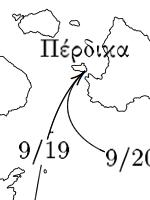
\includegraphics[width=0.2\linewidth]{figs/maps.jpg}
		}
		\hfill
    \subfloat[Musical notes]{%
      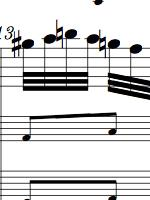
\includegraphics[width=0.2\linewidth]{figs/music.jpg}
		}
		\hfill
    \subfloat[Circular margin]{%
      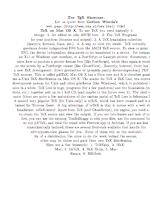
\includegraphics[width=0.2\linewidth]{figs/circular_margin.jpg}
		}
		\hfill
    \subfloat[Tolkien's Tengwar]{%
      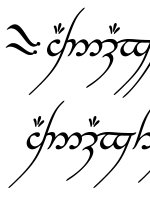
\includegraphics[width=0.2\linewidth]{figs/tengwar.jpg}
		}
	\end{figure}
\end{frame}


\section{Document structure}

\begin{frame}[fragile]
  \begin{columns}
    \begin{column}{0.4\columnwidth}
      \begin{center}
        \LARGE
        name.tex
      \end{center}
    \end{column}
    \begin{column}{0.6\columnwidth}
      \lstinputlisting[language={[latex]tex}]{examples/example1.tex}
    \end{column}
  \end{columns}
\end{frame}

\begin{frame}[fragile]
  \begin{columns}
    \begin{column}{0.4\columnwidth}
      \begin{center}
        \LARGE
        Preamble
      \end{center}
    \end{column}
    \begin{column}{0.6\columnwidth}
      \lstinputlisting[language={[latex]tex},lastline=9]{examples/example1.tex}
    \end{column}
  \end{columns}
\end{frame}

\begin{frame}[fragile]
  \begin{columns}
    \begin{column}{0.4\columnwidth}
      \begin{center}
        \LARGE
        Contents
      \end{center}
    \end{column}
    \begin{column}{0.6\columnwidth}
      \lstinputlisting[language={[latex]tex},firstline=9,firstnumber=9]{examples/example1.tex}
    \end{column}
  \end{columns}
\end{frame}

\begin{frame}
  \begin{figure}
    \includegraphics[height=0.8\textheight]{examples/example1.pdf}
    \caption{Above code compiled to PDF.}
  \end{figure}
\end{frame}


\section{The main contents}

\subsection{Paragraphs and sectioning}

\begin{frame}[fragile]
  \begin{block}{Paragraphs}
    \begin{itemize}
      \item Written as normal text.

      \item Paragraphs separated by empty line.
    \end{itemize}
  \end{block}

  \pause

  \begin{example}
  \begin{lstlisting}
This is a paragraph.

This is another paragraph.
  \end{lstlisting}
  \end{example}
\end{frame}

\begin{frame}
  \begin{block}{Sections}
    \begin{description}
      \item[\textbackslash chapter] Available in bigger classes:
        book, report.

      \item[\textbackslash section] Sections, available in all classes.

      \item[\textbackslash subsection] Subsections, in all classes.

      \item[\textbackslash subsubsection] In most classes.

      \item[\textbackslash paragraph] Named paragraphs, in most classes. 
        Sometimes same as subsubsection.

    \end{description}
  \end{block}
\end{frame}

\begin{frame}[fragile]
  \begin{example}
    \begin{lstlisting}
\section[Short title]{Full title}

This is the text of the first paragraph.

And the second.

\subsection{Subsection title}

And we continue \dots
    \end{lstlisting}
  \end{example}
\end{frame}


\subsection{References}

\begin{frame}[fragile]
  \begin{example}[Input]
    \begin{lstlisting}
...
\usepackage{biblatex}
\addbibresource{literature.bib}
...
According to \textcite{Knuth1997tao} there is no algorithm to solve the 
problem.
...
\printbibliography
    \end{lstlisting}
  \end{example}

  \pause

  \begin{example}[Output]
    \begin{quote}
      According to \textcite{Knuth1997tao} there is no algoritm to solve the 
      problem.
    \end{quote}
  \end{example}
\end{frame}

\begin{frame}[fragile,allowframebreaks]
  \begin{example}[Bib\TeX]
    \lstinputlisting[firstline=38,lastline=46,firstnumber=38]{literature.bib}
  \end{example}
\end{frame}


\subsection{Mathematics}

\begin{frame}[fragile]
  \begin{example}[Input]
    \begin{lstlisting}
We have the sum \(
  \sum_{i=1}^n i = \frac{n (n + 1)}{2}.
\) But then we also have the sum \[
  \sum_{i=1}^n i = \frac{n (n + 1)}{2}.
\]
    \end{lstlisting}
  \end{example}

  \pause

  \begin{example}[Output]
    \begin{quote}
We have the sum \(
  \sum_{i=1}^n i = \frac{n (n + 1)}{2}.
\) But then we also have the sum \[
  \sum_{i=1}^n i = \frac{n (n + 1)}{2}.
\]
    \end{quote}
  \end{example}
\end{frame}

\begin{frame}[fragile]
  \begin{example}[Input]
    \begin{lstlisting}
\[ f(a) = \left\{
  \begin{array}{ll}
    y & \text{if } a=x \\
    x & \text{if } a=y
  \end{array}
  \right\} = f^{-1}(a). \]
    \end{lstlisting}
  \end{example}

  \pause

  \begin{example}[Output]
    \begin{quote}
      \[ f(a) = \left\{
          \begin{array}{ll}
            y & \text{if } a=x \\
            x & \text{if } a=y
          \end{array}
      \right\} = f^{-1}(a). \]
    \end{quote}
  \end{example}
\end{frame}

\begin{frame}
  \begin{remark}[\TeX{} math mode]
    \begin{itemize}
      \item Sometimes you encounter \$ and \$\$ for maths mode.
      \item This is old \TeX{}, avoid it.
    \end{itemize}
  \end{remark}
\end{frame}


\subsection{Figures and tables}

\begin{frame}[fragile]
  \begin{example}[Figures]
    \begin{lstlisting}
\usepackage{graphicx}
...
\begin{figure}
  \centering
  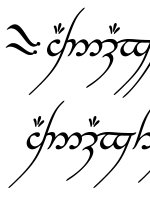
\includegraphics[width=0.2\linewidth]{figs/tengwar.jpg}
  \caption{An example from J.~R.~R.~Tolkien's Tengwar.}
  \label{fig:bild}
\end{figure}
    \end{lstlisting}
  \end{example}
\end{frame}

\begin{frame}
	\begin{figure}
		\centering
    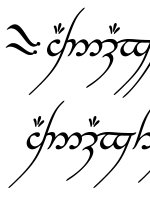
\includegraphics[width=0.2\linewidth]{figs/tengwar.jpg}
    \caption{An example from J.~R.~R.~Tolkien's Tengwar.}
    \label{fig:bild}
	\end{figure}
\end{frame}

\begin{frame}[fragile,allowframebreaks]
	\begin{lstlisting}
\begin{table}
  \centering
  \begin{tabular}{rcccccccccc}
    \toprule
    \(\alpha\) & a & b & c & d & e & f & g & h & i & j \\
    \(P_E(\alpha)\) & 8.2  & 1.5 & 2.8 & 4.3 & 12.7 & 2.2 & 2.0 & 6.1 & 7.0 & 0.2 \\
    \(P_S(\alpha)\) & 9.3  & 1.3 & 1.3 & 4.5 & 9.9 & 2.0 & 3.3 & 2.1 & 5.1 & 0.7 \\
    \bottomrule
  \end{tabular}
  \caption{Table of the probability function for letters of the English and 
  Swedish language, \(P_E\) and \(P_S\), respectively.
  Values are given as per cent with one decimal number precision.}
  \label{tbl:probabilities}
\end{table}
	\end{lstlisting}
\end{frame}

\begin{frame}
\begin{table}
  \centering
  \begin{tabular}{rcccccccccc}
    \toprule
    \(\alpha\) & a & b & c & d & e & f & g & h & i & j \\
    \(P_E(\alpha)\) & 8.2  & 1.5 & 2.8 & 4.3 & 12.7 & 2.2 & 2.0 & 6.1 & 7.0 & 0.2 \\
    \(P_S(\alpha)\) & 9.3  & 1.3 & 1.3 & 4.5 & 9.9 & 2.0 & 3.3 & 2.1 & 5.1 & 0.7 \\
    \bottomrule
  \end{tabular}
  \caption{Table of the probability function for letters of the English and 
  Swedish language, \(P_E\) and \(P_S\), respectively.
  Values are given as per cent with one decimal number precision.}
  \label{tbl:probabilities}
\end{table}
\end{frame}


\subsection{Cross-referencing}

\begin{frame}[fragile]
  \begin{example}
    \begin{lstlisting}
To understand this text you should see Table \ref{tbl:probabilities}.
    \end{lstlisting}
    \begin{lstlisting}
...
\usepackage[swedish]{babel}
\usepackage{cleveref}
...
To understand this text you should see \cref{tbl:probabilities}.
    \end{lstlisting}
  \end{example}
\end{frame}


\section{Useful classes and packages}

\subsection{Some packages}

\begin{frame}
	\begin{description}
    \item[siunitx] Used to correctly typeset units.

    \item[biblatex] Used for reference management.

    \item[listings] Used to list source code.
  \end{description}
\end{frame}

\begin{frame}[fragile]
  \begin{example}[siunitx input]
    \begin{lstlisting}
...
\usepackage[binary-units]{siunitx}
...
A standard ruler is \si{30}{\centi\metre}.
It cannot measure data since that unit is in \SI{\kibi\byte} or 
\si{\kilo\byte}.
    \end{lstlisting}
  \end{example}

  \pause

  \begin{example}
    \begin{quote}
      A standard ruler is \SI{30}{\centi\metre}.
      It cannot measure data since that unit is in \si{\kibi\byte} or 
      \si{\kilo\byte}.
    \end{quote}
  \end{example}
\end{frame}


\subsection{An example document}

\begin{frame}[fragile,allowframebreaks]
  \lstinputlisting{examples/examples.tex}
\end{frame}

\begin{frame}
  \begin{figure}
    \includegraphics[height=0.8\textheight]{examples/examples.pdf}
    \caption{The result}
  \end{figure}
\end{frame}


\subsection{Slides in beamer}

%\begin{frame}[allowframebreaks]{beamer}
%	\lstinputlisting{latex.tex}
%\end{frame}

\begin{frame}
  \begin{remark}
    \begin{itemize}
      \item Run \lstinline{texdoc beamer} in the terminal.
      \item This will show you 
        \citetitle{beameruserguide}~\cite{beameruserguide}.
    \end{itemize}
  \end{remark}
\end{frame}

